\chapter{Background}

\section{Model Checking}
Model checking.~\cite{modelChecking} is a crucial concept when it comes to hardware and software verification as it gives the basis for all possible solutions. 
It is a widely used method for formal software verification which main aim is to provide a mathematically precise proof for the correctness of a program. By exhaustively traversing through every possible execution of the program for every possible input, it checks whether a certain property was satisfied. 
The main property during this paper was reachability, which means we explore the state space of a program to see if a certain bad state can be reached.

\begin{figure}
  \centering
  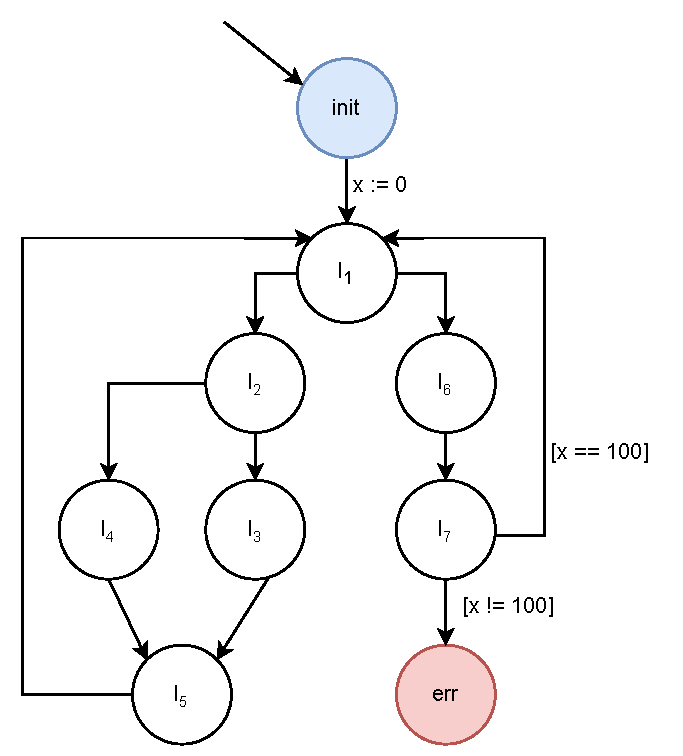
\includegraphics[width=0.5\textwidth]{figures/cfa_simple.pdf}
  \caption{Simple representation of a Control-Flow Automata (CFA).}
  \label{fig:cfa}
\end{figure}

To perform model checking, the program code needs to be represented in a way that makes its control and data flow analyzable. A widely used formalism is the \textbf{Control-Flow Automata (CFA)}~\cite{cfa}. Figure~\ref{fig:cfa} illustrates a simplified CFA, which models how control moves between different parts of a program.

A CFA is a graph-based representation of the program and consists of:
\begin{itemize}
  \item \textbf{Locations} — These represent program points (e.g., line numbers or steps) and are shown as circles in the figure. The blue circle denotes the \textit{initial state}, and the red circle marks the \textit{error state}.
  \item \textbf{Edges} — These indicate transitions between locations and represent operations such as assignments or conditional checks. In the figure, they are visualized as arrows.
\end{itemize}

It helps in analyzing programs, especially for checking if errors (like reaching a bad state) can happen. In this documentation, I will describe how a BTOR2 program can be transformed into a CFA, and how this representation supports effective model checking.

\section{BTOR2}
The Hardware Model Checking Competition (HWMCC)~\cite{hwmcc} serves as a benchmark for evaluating formal verification tools for hardware systems. A key innovation supporting this effort is BTOR2~\cite{btor2}, a word-level model checking format designed for bit-precise modeling of word-level sequential circuits.
The BTOR2 language extends the previous bit-level AIGER~\cite{AIGER} format with higher-level abstractions, making it ideal for various verification techniques. It introduces a simple, sorted, line-based syntax that is easy to parse and aligns with SMT-LIB~\cite{SMT-LIB} semantics for bit-vectors and arrays.

\begin{figure}
  \centering
  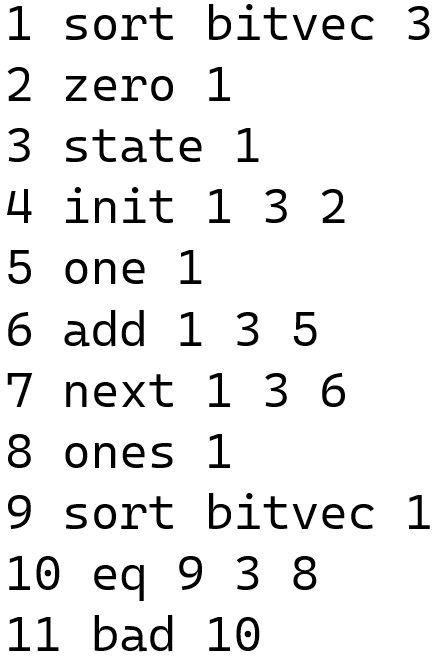
\includegraphics[width=0.2\textwidth]{figures/count2.png}
  \caption{ Syntax of Btor2. count2.btor2 example. }
  \label{fig:count2}
\end{figure}

In Figure~\ref{fig:count2} is a BTOR2 circuit that defines a simple finite state machine -- a 3-bit counter -- that starts from zero and increments by one at each time step. Each line defines a node in the circuit, such as a constant, state, operation, or property.

At the beginning of the circuit, line 1 declares a bit-vector of width 3 \verb|sort bitvec 3|, which serves as the type for all 3-bit values used throughout the circuit. This will have a sort id or \verb|sid| of '1' which will be used to declare registers and operations.

Line 2 defines a constant zero \verb|zero 1|, which produces the bit-vector \verb|000| and has a node id or \verb|nid| of '2'. Following this, line 3 introduces a state variable of sort 1 (3 bits), representing the main state of the circuit.

The initial value of state '3' is specified in line 4, which uses the init keyword to bind state 3 to start at constant 2, which is the \verb|000| bit-vector. The next input is defined in line 5 using one 1, which denotes the constant \verb|001|.

Line 6 defines an addition operation that adds 1 to the main state, resulting in node 6, the next value of the counter. This operation wraps around on overflow due to the fixed 3-bit width. Line 7 then uses the next keyword to specify that in the next state, the counter should take the value of node 6, i.e., the incremented result.

To define a property of interest, line 8 declares another constant: \verb|ones 1|, which represents the maximum value a 3-bit counter can hold—namely \verb|111|. Line 9 introduces a new sort of width 1, which is used for boolean-like signals such as equality checks.

Line 10 defines a comparison between the current counter value and the maximum value \verb|111| using the eq operator. This operation returns a 1-bit result: true (1) if the counter is at maximum, false (0) otherwise. Finally, line 11 marks this equality result as a bad state, which is a safety property violation. Hence, the circuit asserts that reaching the value 111 is undesirable or erroneous.

In summary, this BTOR2 circuit models a 3-bit counter that increments with each step and triggers a bad state when it reaches 111. This design could be used in formal verification to prove that the system avoids overflow, or alternatively, to find the point at which it does. The clear structure and modular nature of BTOR2 make it suitable for such sequential hardware modeling and property checking.

\subsection{Btor2C}
Btor2C~\cite{btor2c} is a tool that translates Btor2 hardware models into equivalent C programs. This allows software verification tools to analyze hardware designs, bridging the gap between hardware and software verification.
In my implementation, I focused on bit-vectors and their related functions and definitions, leveraging the expressive power of BTOR2 to model and verify small, bit-precise sequential systems.

\section{Theta}
Regarding the implementation, I chose Theta~\cite{theta}, a modular and extensible model checking framework developed by the Critical Systems Research Group at the Budapest University of Technology and Economics, as the target platform for integrating a BTOR2 frontend.
To begin, I defined an unofficial BTOR2 grammar using ANTLR4~\cite{antlr}, a powerful parser generator widely adopted in both academia and industry for constructing interpreters, compilers, and domain-specific languages.
Theta natively supports abstraction-refinement based reachability analysis. In my project, I worked with XCFA models—an extension of Control Flow Automata (CFA) that incorporates procedures and concurrency - but focused primarily on the CFA subset. This allowed me to apply Theta's robust CEGAR-based algorithms for reachability checking.